\documentclass{gescons}

\genre {Entrevista}
\author{Wanderley Carvalho}
\title{Tanatofobia: Da Ressignificação da Existência à~Superação do Medo da Morte}
\paginaurl{https://www.youtube.com/live/OEjbTVk1zuY}

\begin{document}
    \makeentrevistatitle
    \coverart{back/Wanderley_Carvalho}

    \begin{multicols}{2}

\begin{center}
    \vspace{-0.5cm}
    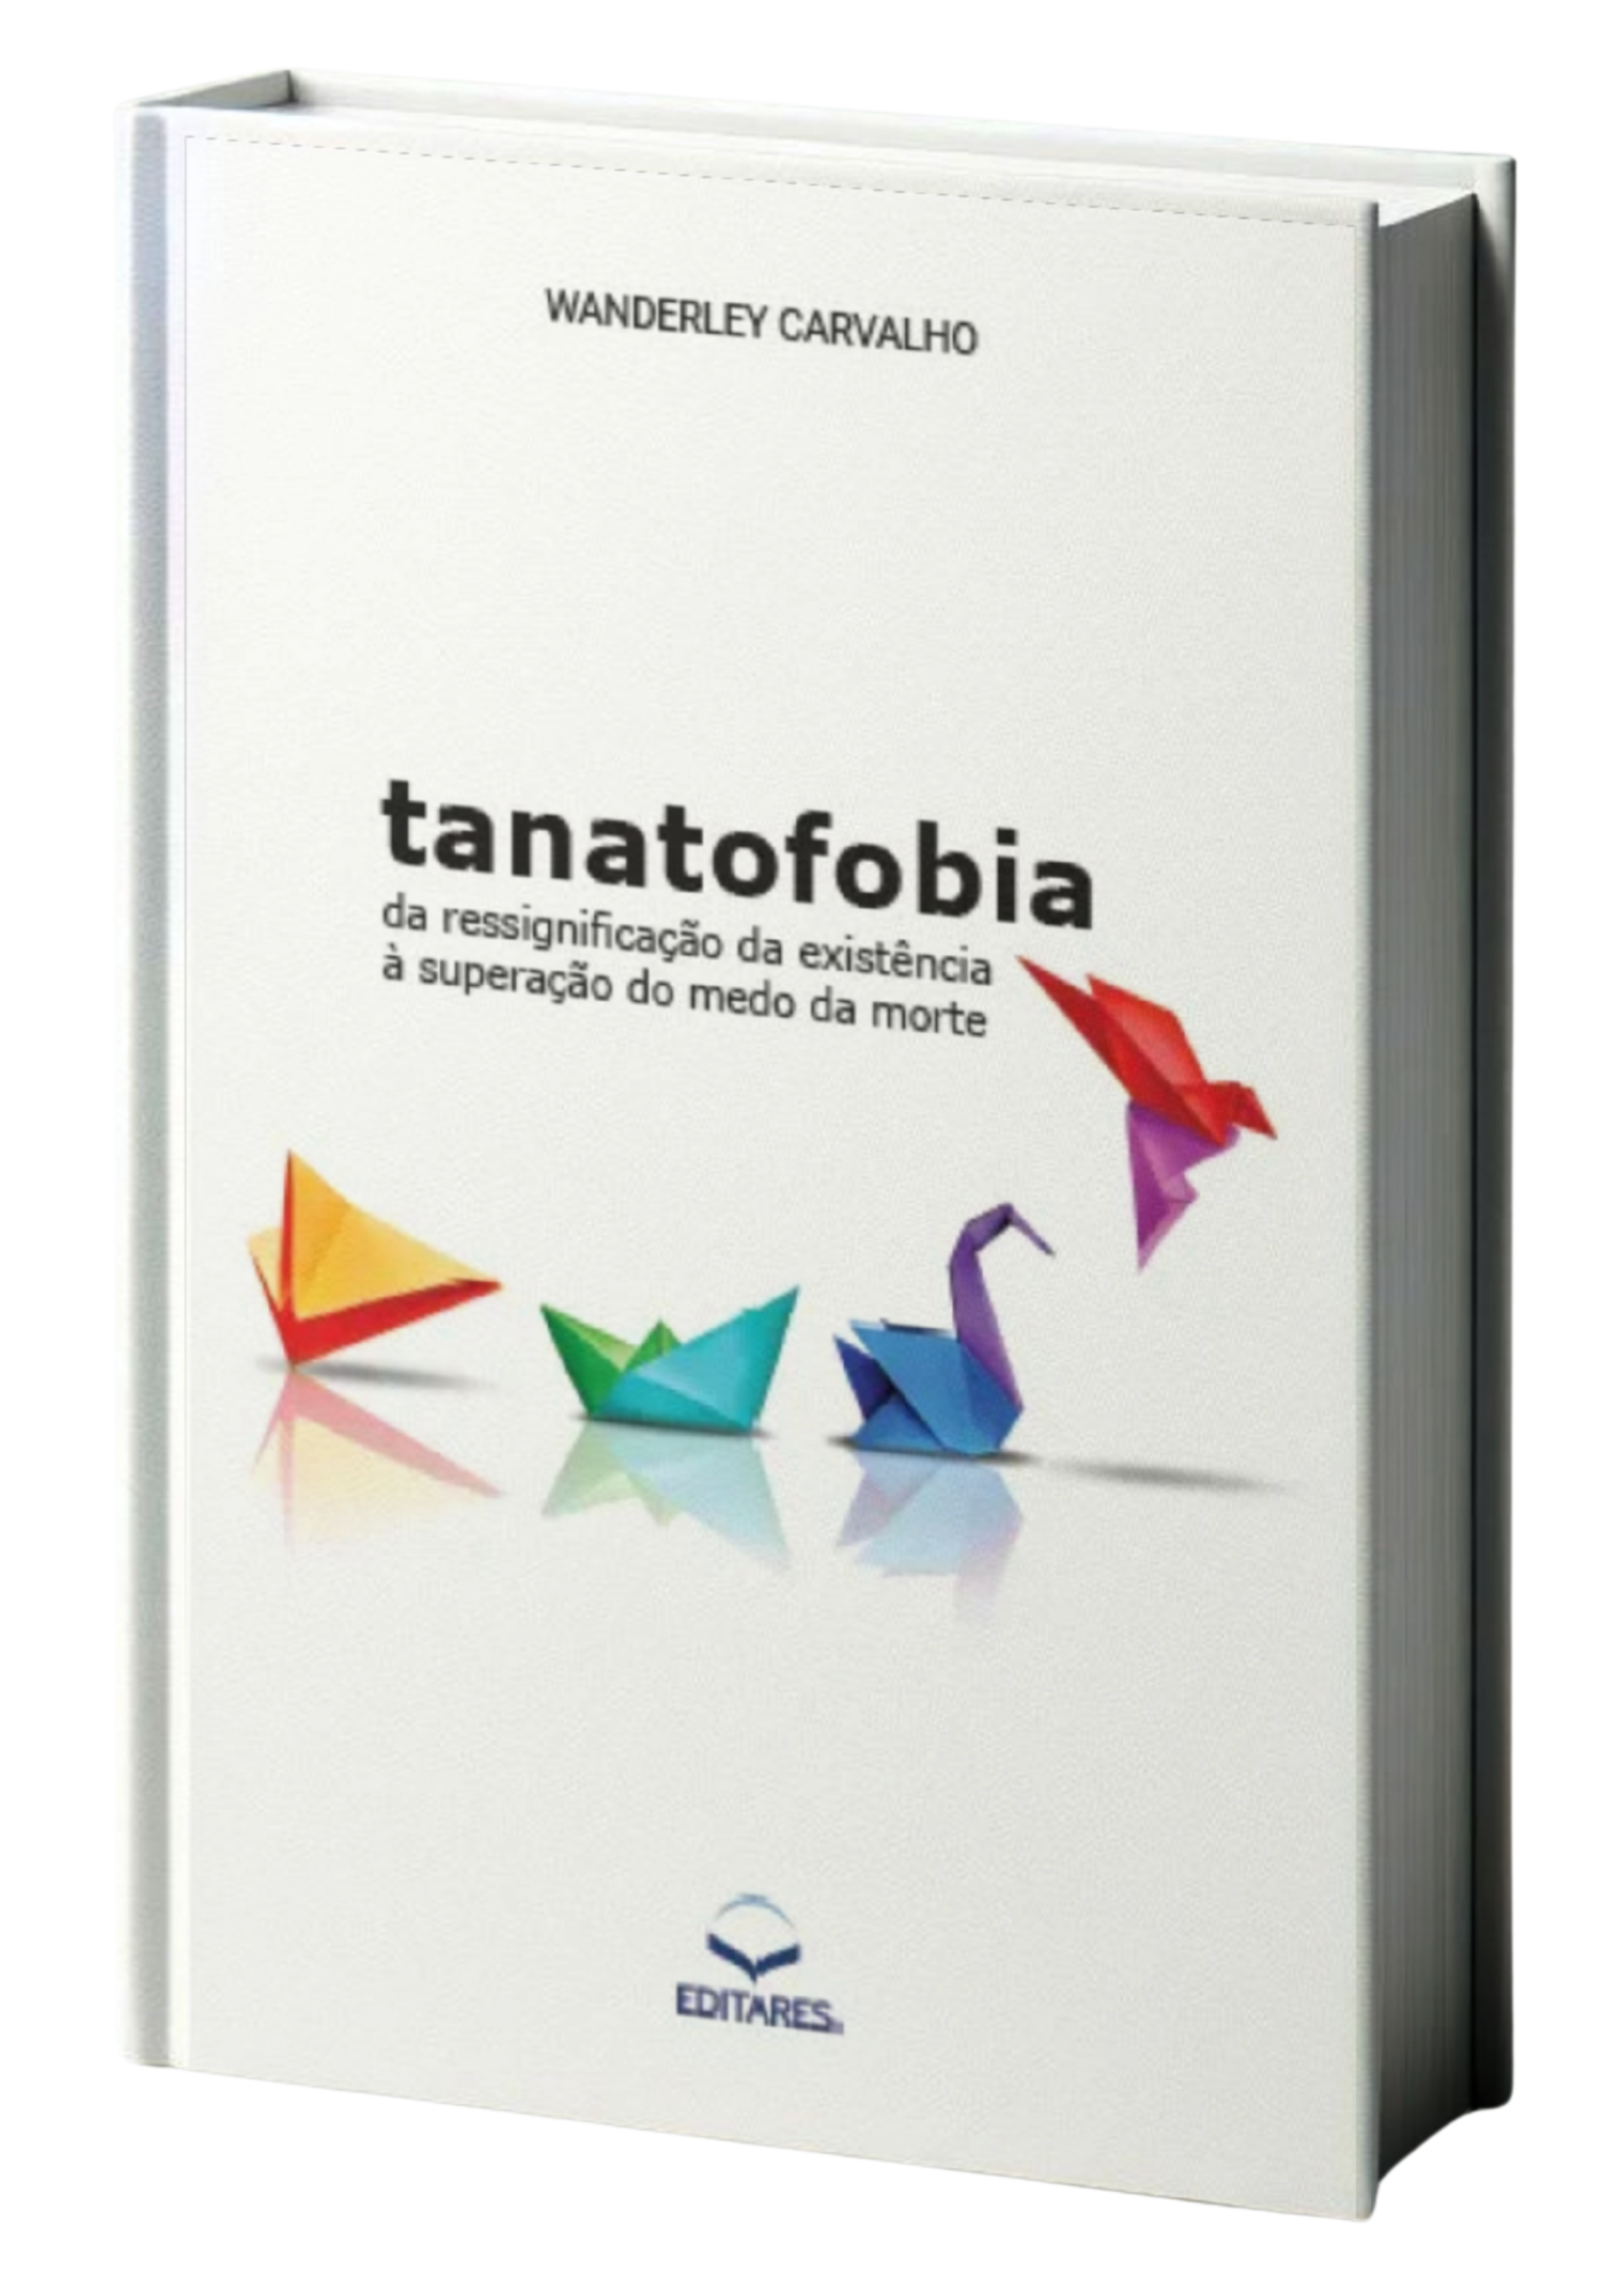
\includegraphics[width=6cm]{articles/entrevista/mockups/Wanderley_Carvalho.png}
\end{center}


\textbf{1. Qual foi a~motivação para a~escrita da obra? Por que a~definição deste tema para publicação de um livro?}


A tanatofobia, aversão patológica a~um ou mais aspectos relacionados à~morte biológica de si ou de outrem, ocupa posição destacada entre as aflições humanas, sendo considerada por muitos o~maior dos quadros fóbicos a~acometer nossa espécie. Pesquisas demonstram haver forte tendência de os grupos humanos lançarem mão de diversos mecanismos, visando negar ou mascarar a~finitude, em claro movimento de fuga da realidade.

Práticas culturais de diversas ordens, seja no âmbito familiar, seja no seio da sociedade, podem atuar na difusão de concepções estreitas, equivocadas, dogmáticas e~aterrorizantes desse fenômeno indissociável da vida, promovendo perpetuação de quadros tanatofóbicos ao longo da série existencial da consciência. Desse modo, a~obra tem o~objetivo precípuo de prestar esclarecimento para prevenção ou superação do problema.

\textbf{2. Quais foram as principais percepções, intra e~extrafísicas, durante a~pesquisa e~a~escrita da obra? E~posterior ao lançamento?}

Merecem destaque as inúmeras sincronicidades experimentadas por ocasião tanto da investigação quanto da escrita, além da evidente atuação do amparo de função. Após o~lançamento, o~aspecto mais expressivo foram os \emph{insights} e~oportunidades para realização de nova pesquisa, desta vez, visando publicação em coautoria.

\textbf{3. Qual o~maior aprendizado com a~escrita desta obra?}

O verdadeiro mergulho no tema proporcionou a~este autor -- além do esperado aprofundamento conceitual em torno da problemática, das causas e~manifestações da tanatofobia e~dos recursos de superação e~prevenção desta -- autorreciclagem intraconsciencial gradativa, muitas vezes perpceptível após decorrido considerável intervalo temporal.

\begin{pullquote}
    ``O verdadeiro mergulho no tema proporcionou a~este autor  (...)  autorreciclagem intraconsciencial gradativa, muitas vezes perpceptível após decorrido considerável intervalo temporal.''
\end{pullquote}

\textbf{4. O~que poderia dizer como incentivo para que mais pesquisadores invistam na publicação de obras conscienciológicas?}

Aos pesquisadores ainda não envolvidos em gescon-livro, deixo aqui o~convite para que o~façam, dado o~grande potencial de realizar esclarecimento exibido pelas obras conscienciológicas.



    \end{multicols}
\end{document}
